\documentclass[12pt]{article}
\usepackage[margin=0.85in]{geometry}
\usepackage{amsmath,amssymb}
\usepackage{enumerate}
\usepackage{tikz}
\usetikzlibrary{trees}
\pagestyle{empty}
\setlength{\parindent}{0pt}
\setlength{\parskip}{3pt}

\tikzset{
  dec/.style={circle,fill,inner sep=1.5pt},
  gametree/.style={level distance=12mm, every node/.style={font=\small}},
  opt/.style={line width=1.5pt}
}

\begin{document}

\begin{center}
{\large Problem set 2 -- Econ 5030}
\end{center}

%%%%%%%%%%%%%%%%%%%%%%%%%%%%%%%%%%%%%%%%%%%%%%%%%%%%%%%%%%%%%%%%%%%%%%%
\textbf{1. Iterated deletion}

\textbf{A)} R1: $n_G$ str.\ dom.\ by $l_G$ ($3>0,1,1$); $n_P$ str.\ dom.\ by $l_P$ ($2>0$, $3>1$, $3>1$). ($h_P$ vs $l_P$ only weak: tie $2=2$ at $n_G$.)
R2: $h_G$ str.\ dom.\ $l_G$ ($4>3$, $5>3$); $h_P$ str.\ dom.\ $l_P$ ($4>3$, $5>3$).
Solution set: $\{(h_G,h_P)\}$, payoffs $(5,5)$.

\textbf{B)} $BR_G$: $n_P\to l_G$, $l_P\to h_G$, $h_P\to h_G$. $BR_P$: $n_G\to\{l_P,h_P\}$, $l_G\to h_P$, $h_G\to h_P$. NE $=\{(h_G,h_P)\}$ (unique, also in mixed, since dominance solvable).

%%%%%%%%%%%%%%%%%%%%%%%%%%%%%%%%%%%%%%%%%%%%%%%%%%%%%%%%%%%%%%%%%%%%%%%
\medskip
\textbf{2. Normal form}

\textbf{1.} Tree, payoffs $(u_1,u_2)$; thick = backward induction.
\begin{center}
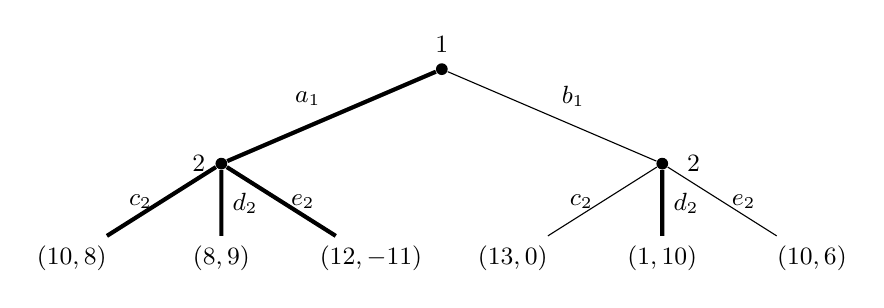
\begin{tikzpicture}[gametree,
  level 1/.style={sibling distance=56mm},
  level 2/.style={sibling distance=19mm}]
\node[dec,label=above:{1}] {}
  child { node[dec,label=left:{2\ }] {}
    child { node {$(10,8)$} edge from parent node[left] {$c_2$} }
    child { node {$(8,9)$} edge from parent[opt] node[right] {$d_2$} }
    child { node {$(12,-11)$} edge from parent node[right] {$e_2$} }
    edge from parent[opt] node[above left] {$a_1$} }
  child { node[dec,label=right:{\ 2}] {}
    child { node {$(13,0)$} edge from parent node[left] {$c_2$} }
    child { node {$(1,10)$} edge from parent[opt] node[right] {$d_2$} }
    child { node {$(10,6)$} edge from parent node[right] {$e_2$} }
    edge from parent node[above right] {$b_1$} };
\end{tikzpicture}
\end{center}

\textbf{2.} $S_1=\{a_1,b_1\}$. $S_2=\{xy: x,y\in\{c_2,d_2,e_2\}\}$, $x$ after $a_1$, $y$ after $b_1$ (9 strategies).

\textbf{3.}
\begin{center}
\small
\setlength{\tabcolsep}{3.5pt}
\begin{tabular}{r|ccccccccc}
 & $cc$ & $cd$ & $ce$ & $dc$ & $dd$ & $de$ & $ec$ & $ed$ & $ee$ \\ \hline
$a_1$ & $10,8$ & $10,8$ & $10,8$ & $8,9$ & $8,9$ & $8,9$ & $12,-11$ & $12,-11$ & $12,-11$ \\
$b_1$ & $13,0$ & $1,10$ & $10,6$ & $13,0$ & $1,10$ & $10,6$ & $13,0$ & $1,10$ & $10,6$
\end{tabular}
\end{center}

\textbf{4.} Vs $a_1$: P2 needs $d_2$ after $a_1$ ($9>8>-11$); then $a_1$ (8) $\ge$ $b_1$ only if $y=d_2$ ($13,1,10$). Vs $b_1$: P2 needs $d_2$ after $b_1$; then $b_1$ gives $1<10,8,12$. Unique pure NE: $(a_1, d_2d_2)$, payoffs $(8,9)$.

\textbf{5.} No. Backward induction: $d_2$ after $a_1$, $d_2$ after $b_1$ ($10>6>0$); P1: $8>1\Rightarrow a_1$. SPE $=(a_1,d_2d_2)=$ the NE. The punishment $d_2$ after $b_1$ is P2's best reply there, so the threat is credible.

%%%%%%%%%%%%%%%%%%%%%%%%%%%%%%%%%%%%%%%%%%%%%%%%%%%%%%%%%%%%%%%%%%%%%%%
\medskip
\textbf{3. Timing and strategies}

\textbf{2.1} No info: strategy = action. $S_1=S_2=\{0,1\}$; $2\times2$ matching pennies, no pure NE, mixed $(\tfrac12,\tfrac12)$.

\textbf{2.2} $S_1=\{0,1\}$. P2 conditions on P1's move: $S_2=\{(0,0),(0,1),(1,0),(1,1)\}$ ($x$ after 0, $y$ after 1) = always 0, copy, opposite, always 1.

\textbf{2.3} Same actions, different strategy sets: $2\times2$ vs $2\times4$.
\begin{center}
\begin{tabular}{r|cccc}
 & $(0,0)$ & $(0,1)$ & $(1,0)$ & $(1,1)$ \\ \hline
$0$ & $1,0$ & $1,0$ & $0,1$ & $0,1$ \\
$1$ & $0,1$ & $1,0$ & $0,1$ & $1,0$
\end{tabular}
\end{center}
Timing/info enter only through strategy sets. Sequential: P2's ``opposite'' $(1,0)$ always wins; NE $=(0,(1,0)),(1,(1,0))$, payoffs $(0,1)$. Simultaneous: each wins w.p.\ $\tfrac12$.

%%%%%%%%%%%%%%%%%%%%%%%%%%%%%%%%%%%%%%%%%%%%%%%%%%%%%%%%%%%%%%%%%%%%%%%
\medskip
\textbf{4. Third party observation}

\textbf{2.4} No. With payoff $=$ own \$, $(M,M)$ is not NE: vs $M$, deviate to $L$ ($\$30>\$18$) if first \$ is the row player's, or to $H$ ($\$20>\$18$) if first \$ is P1's. This rejects ``maximize own money $+$ NE'', not game theory: payoffs are utilities over outcomes, and the experimenter controls money, not preferences.

\textbf{2.5} $G=(N,\{S_i\},\{u_i\})$: players; strategies $=$ complete contingent plans (an action at every info set, even unreached); $u_i:\prod_j S_j\to\mathbb{R}$ represents $i$'s preferences over induced outcomes (ordinal for pure, vNM for mixed). Players choose strategies simultaneously and independently; timing/info appear only through $S_i$. Here $S_i=\{L_i,M_i,H_i\}$ and $u_i$ need not equal own \$.

\textbf{2.6} Fairness/social preferences: $u_i=x_1+x_2+\min\{x_1,x_2\}$ (same for both players).
\begin{center}
\begin{tabular}{r|ccc}
 & $L_1$ & $M_1$ & $H_1$ \\ \hline
$L_2$ & $24,24$ & $50,50$ & $17,17$ \\
$M_2$ & $50,50$ & $54,54$ & $28,28$ \\
$H_2$ & $17,17$ & $28,28$ & $15,15$
\end{tabular}
\end{center}
$M$ strictly dominant ($50>24,17$; $54>50,28$; $28>17,15$) $\Rightarrow$ unique NE $(M_1,M_2)$.

\textbf{Rationality test?} No, not alone. Utilities are unobserved and any profile can be made the unique NE by choice of preferences (as in 2.6). The data only test rationality jointly with an assumed utility (e.g.\ own money). Need cross-game consistency (revealed preference) or elicited preferences/beliefs.

%%%%%%%%%%%%%%%%%%%%%%%%%%%%%%%%%%%%%%%%%%%%%%%%%%%%%%%%%%%%%%%%%%%%%%%
\medskip
\textbf{5. SPNE} (P2 observes P1, then picks $U_2/D_2$.)

\textbf{1.} $S_1=\{L_1,M_1,H_1\}$; $S_2=\{U,D\}^3$, $x_Lx_Mx_H$ = action after $L_1,M_1,H_1$ (8 strategies); $u_i(k_1,x_Lx_Mx_H)=u_i(k_1,x_k)$.

\textbf{2.}
\begin{center}
\small
\setlength{\tabcolsep}{3.5pt}
\begin{tabular}{r|cccccccc}
 & $UUU$ & $UUD$ & $UDU$ & $UDD$ & $DUU$ & $DUD$ & $DDU$ & $DDD$ \\ \hline
$L_1$ & $10,10$ & $10,10$ & $10,10$ & $10,10$ & $1,11$ & $1,11$ & $1,11$ & $1,11$ \\
$M_1$ & $5,5$ & $5,5$ & $2,6$ & $2,6$ & $5,5$ & $5,5$ & $2,6$ & $2,6$ \\
$H_1$ & $1,4$ & $3,5$ & $1,4$ & $3,5$ & $1,4$ & $3,5$ & $1,4$ & $3,5$
\end{tabular}
\end{center}
P2 plays $D$ on path ($11>10$, $6>5$, $5>4$). $L_1$: gets 1 $<$ $M_1$'s $\ge 2$, no NE. $M_1$: need $x_L=D$, $x_H=U$. $H_1$: need $x_L=x_M=D$.
NE: $(M_1,DDU)$ $(2,6)$ and $(H_1,DDD)$ $(3,5)$.

\textbf{3.}
\begin{center}
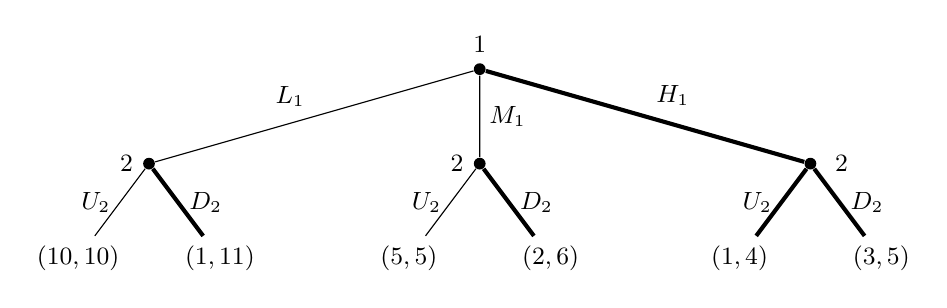
\begin{tikzpicture}[gametree,
  level 1/.style={sibling distance=42mm},
  level 2/.style={sibling distance=18mm}]
\node[dec,label=above:{1}] {}
  child { node[dec,label=left:{2\ }] {}
    child { node {$(10,10)$} edge from parent node[left] {$U_2$} }
    child { node {$(1,11)$} edge from parent[opt] node[right] {$D_2$} }
    edge from parent node[above left] {$L_1$} }
  child { node[dec,label=left:{2\ }] {}
    child { node {$(5,5)$} edge from parent node[left] {$U_2$} }
    child { node {$(2,6)$} edge from parent[opt] node[right] {$D_2$} }
    edge from parent node[right] {$M_1$} }
  child { node[dec,label=right:{\ 2}] {}
    child { node {$(1,4)$} edge from parent node[left] {$U_2$} }
    child { node {$(3,5)$} edge from parent[opt] node[right] {$D_2$} }
    edge from parent[opt] node[above right] {$H_1$} };
\end{tikzpicture}
\end{center}
P2: $D_2$ at every node. P1: $1,2,3\Rightarrow H_1$. SPE: $(H_1,DDD)$, payoffs $(3,5)$. $(M_1,DDU)$ is not SPE: it uses the incredible threat $U_2$ after $H_1$ ($4<5$).

\end{document}
